\documentclass[12pt]{ctexart}
    %%% Document Settings %%%%
%\usepackage[utf8]{inputenc}

\usepackage[
    twoside,
    top=1in,
    bottom=0.75in,
    inner=0.5in,
    outer=0.5in,
]{geometry}
\pagestyle{myheadings}
\usepackage{minted}
\usepackage[dvipsnames,svgnames]{xcolor}

%%%% Additional Commands to Load %%%%
\usepackage{tcolorbox}
\tcbuselibrary{skins}
\tcbuselibrary{minted}
\usemintedstyle{lovelace}
%\usepackage{minted}
\usepackage{color}
\usepackage{tikz}
\usetikzlibrary{calc}
\usepackage{tabularx,colortbl}
\usepackage{amsfonts,amsmath,amssymb}
\usepackage{titling}
\usepackage{mathrsfs}
\usepackage{calc}
\usepackage{subcaption}

\usepackage{listings}
%\usepackage{newtxtext}
\usepackage[strict]{changepage} 
\usepackage{framed}
\definecolor{formalshade}{rgb}{0.95,0.95,1}
\usepackage{float}

%%%% Commands to Define Homework Boxes %%%%
%%%% Box Definition %%%%
\newtcolorbox{prob}[1]{
% Set box style
    sidebyside,
    sidebyside align=top,
% Dimensions and layout
    width=\textwidth,
    toptitle=2.5pt,
    bottomtitle=2.5pt,
    righthand width=0.20\textwidth,
% Coloring
    colbacktitle=gray!30,
    coltitle=black,
    colback=white,
    colframe=black,
% Title formatting
    title={
        #1 \hfill Grade:\phantom{WWWW}
    },
    fonttitle=\large\bfseries
}

%%%% Environment Definition %%%%
\newenvironment{problem}[1]{
    \begin{prob}{#1}
}
{
    \tcblower
    \centering
    \textit{\scriptsize\bfseries Faculty Comments}
    \vspace{\baselineskip}
    \end{prob}
}

\newenvironment{formal}{%
\def\FrameCommand{%
\hspace{1pt}%
{\color{DarkBlue}\vrule width 2pt}%
{\color{formalshade}\vrule width 4pt}%
\colorbox{formalshade}%
}%
\MakeFramed{\advance\hsize-\width\FrameRestore}%
\noindent\hspace{-4.55pt}% disable indenting first paragraph
\begin{adjustwidth}{}{7pt}%
\vspace{2pt}\vspace{2pt}%
}
{%
\vspace{2pt}\end{adjustwidth}\endMakeFramed%
}

    \title{特殊方程作业8}
    \author{地物2201班\ 杨曜堃}
    \date{\today}
%%% document
\begin{document}

% Format Running Header
    \markboth{\theauthor}{\thetitle}
    \maketitle
    \begin{description}
        \item[问题1] 设$u(x,t)$满足波动方程的Cauchy问题$$
        \begin{cases}
            \dfrac{\partial^2u}{\partial t^2}=\dfrac{\partial^2u}{\partial x^2},&\quad-\infty<x<+\infty,\ t>0\\
            u|_{t=0}=\varphi(x)\\
            \left.\dfrac{\partial u}{\partial t}\right|_{t=0}=\phi(x)
        \end{cases}
        $$
        \begin{enumerate}
            \item 写出形式解(即D'Alembert解);
            \item $\varphi(x)$与$\phi(x)$满足何条件时,仅由左行波构成?
            \item $\varphi(x)$与$\phi(x)$满足何条件时,仅由右行波构成?
            \item 若当$|x|\geqslant10$时初值为0,那么$t$为何值时,$u(-10,t)$不受初始扰动的影响?
        \end{enumerate}
    \end{description}
    \begin{problem}{问题\#1.1}
        由波动方程的行波法,可以得到达朗贝尔公式
        $$
        u(x,t)=\dfrac{1}{2}\varphi(x+t)+\dfrac{1}{2}\varphi(x-t)+\dfrac{1}{2}\int^{x+t}_{x-t}\phi(s)\text{d}s
        $$
    \end{problem}
    \begin{problem}{问题\#1.2}
        由题1.1解出的答案,可以得知,当
        $$
        \phi(x)=\varphi'(x)
        $$
        可以解出$u(x,t)=\varphi(x+t)$,即仅有左行波。
    \end{problem}
    \begin{problem}{问题\#1.3}
        由题1.1解出的答案,可以得知,当
        $$
        \phi(x)=-\varphi'(x)
        $$
        可以解出$u(x,t)=\varphi(x-t)$,即仅有右行波。
    \end{problem}
    \begin{problem}{问题\#1.4}
        采用图解法,如图所示
        \begin{center}
            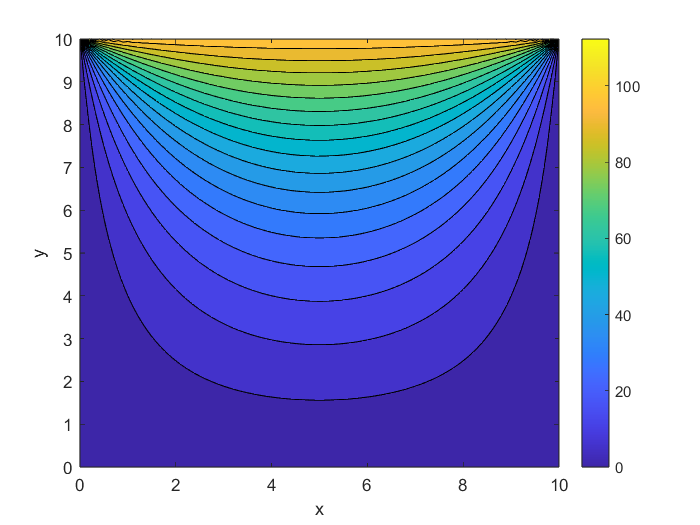
\includegraphics[width=10cm]{fig1.png}
        \end{center}
        可得当$t<10$或$t>30$时,不受初始扰动的影响。
    \end{problem}
    % \begin{lstlisting}[language = Matlab,title={test4\_script.m},  numbers=left, 
    %     numberstyle=\tiny,keywordstyle=\color{blue!70},
    %     commentstyle=\color{red!50!green!50!blue!50},frame=shadowbox,
    %     rulesepcolor=\color{red!20!green!20!blue!20},basicstyle=\ttfamily]
    % \end{lstlisting}
    % \begin{figure}[htbp]
    %     \small
    %     \centering
    %     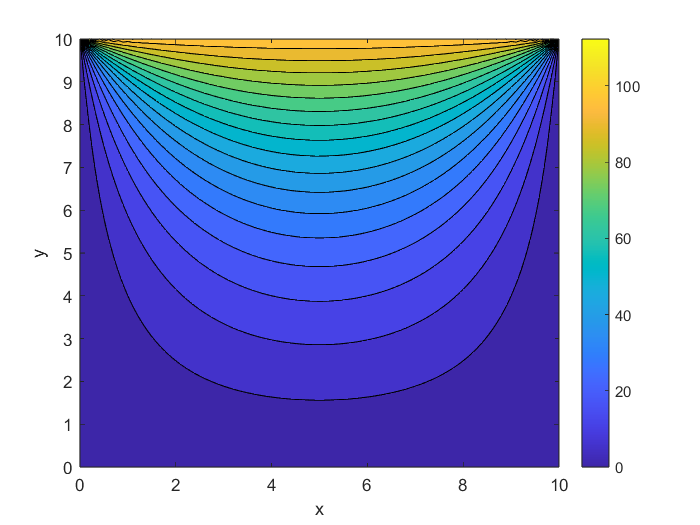
\includegraphics[width=16cm]{fig1.png}
    %     \caption{第一题结果图} \label{Fig:aa}
    % \end{figure}
\end{document}